\documentclass{sig-alternate-05-2015}
\usepackage{pgf}
\usepackage{tikz}
\usetikzlibrary{arrows,automata, positioning}
\usepackage{graphicx}
\usepackage{url}
\usepackage{enumitem}
\usepackage{caption}
\usepackage{listings}
\usepackage{textcomp}
\lstset{basicstyle=\ttfamily, 
        captionpos=b, 
        escapeinside={<@}{@>}}

\usepackage{xcolor}

\newcommand\todo[1]{\textbf{\textcolor{red}{#1}}}
\newcommand{\lstul}[1]{\underline{\mbox{\tt #1}}}

\toappear{}
\begin{document}

% Copyright
\setcopyright{acmcopyright}
%\setcopyright{acmlicensed}
%\setcopyright{rightsretained}
%\setcopyright{usgov}
%\setcopyright{usgovmixed}
%\setcopyright{cagov}
%\setcopyright{cagovmixed}


% DOI
\doi{10.475/123_4}

% ISBN
\isbn{123-4567-24-567/08/06}

%Conference
\conferenceinfo{PLDI '13}{June 16--19, 2013, Seattle, WA, USA}

\acmPrice{\$15.00}

%
% --- Author Metadata here ---
\conferenceinfo{WOODSTOCK}{'97 El Paso, Texas USA}
%\CopyrightYear{2007} % Allows default copyright year (20XX) to be over-ridden - IF NEED BE.
%\crdata{0-12345-67-8/90/01}  % Allows default copyright data (0-89791-88-6/97/05) to be over-ridden - IF NEED BE.
% --- End of Author Metadata ---

\title{Automatic Trigger Generation for Rule-based Smart Homes}
%
% You need the command \numberofauthors to handle the 'placement
% and alignment' of the authors beneath the title.
%
% For aesthetic reasons, we recommend 'three authors at a time'
% i.e. three 'name/affiliation blocks' be placed beneath the title.
%
% NOTE: You are NOT restricted in how many 'rows' of
% "name/affiliations" may appear. We just ask that you restrict
% the number of 'columns' to three.
%
% Because of the available 'opening page real-estate'
% we ask you to refrain from putting more than six authors
% (two rows with three columns) beneath the article title.
% More than six makes the first-page appear very cluttered indeed.
%
% Use the \alignauthor commands to handle the names
% and affiliations for an 'aesthetic maximum' of six authors.
% Add names, affiliations, addresses for
% the seventh etc. author(s) as the argument for the
% \additionalauthors command.
% These 'additional authors' will be output/set for you
% without further effort on your part as the last section in
% the body of your article BEFORE References or any Appendices.

\numberofauthors{2} %  in this sample file, there are a *total*
% of EIGHT authors. SIX appear on the 'first-page' (for formatting
% reasons) and the remaining two appear in the \additionalauthors section.
%
\author{
% 1st. author
\alignauthor
Chandrakana Nandi\\
       \affaddr{University of Washington, Seattle}\\
       \email{cnandi@cs.washington.edu}
\alignauthor Michael D. Ernst\\
       \affaddr{University of Washington, Seattle}\\
       \email{mernst@cs.washington.edu}
%Anonymous submission
}

\maketitle
\begin{abstract}
To customize the behavior of a smart home, an end user writes rules.
When an external event satisfies the rule's trigger, the rule's action executes; for example, when
the temperature is above a certain threshold, then window awnings might be extended.
End users often write incorrect rules~\cite{Huang}.
This paper's technique prevents a certain type of mistake in the rules:  
\textit{errors due to too few triggers}.
It statically analyzes a rule's actions to determine what triggers are necessary. 

We have implemented the technique in the form of a tool called TrigGen and tested it on 116 end-user written
rules for openHAB, an open-source home automation platform.
It identified that 66\% of the rules had fewer triggers than required
for correct behavior.
The missing triggers could lead to unexpected behavior
and security vulnerabilities in a smart home.

\end{abstract}

\printccsdesc


\keywords{Security, Home automation, Trigger action programming, Static analysis}

\section{Introduction}
Most home automation platforms support end-user customization components: a
user writes rules to determine what actions should be taken by what device
under what conditions~\cite{Newmannowwere}. For example, Samsung
SmartThings~\cite{samsung} allows users to create their own automation
rules through their ``SmartApps" feature, while Apple
HomeKit~\cite{homekit} allows users to set conditions that
govern when an action should take place.

A rule has two main components:
triggers that cause a rule to be fired and actions to be executed when a
rules fires. This is also called Trigger Action Programming
(TAP)~\cite{practical-tap}. Listing~\ref{lst:rule} shows an example of a rule. The part between
\texttt{when} and \texttt{then} is the trigger block and the part between
\texttt{then} and \texttt{end} is the action block. There can be multiple
triggers in the trigger part---if one or more is satisfied, the rule is
fired.
A rule engine fires the rules when its triggers are satisfied.

\begin{lstlisting}[caption={A rule that updates the maximum and minimum temperature values for a day---it compares the current temperature with the values starting from midnight of the respective day. },label={lst:rule}]
rule "Update max and min temperatures"
when
 // trigger block	
 Item Temperature changed
then	
 // action block 
 postUpdate(Temp_Max, 
   Temperature.maxSince(now.toDateMidnight))
 postUpdate(Temp_Min, 
   Temperature.minSince(now.toDateMidnight))
end
\end{lstlisting}

Even though TAP is the most commonly used and practical approach for home
automation~\cite{practical-tap, dey}, end users often make errors in writing
trigger-action programs~\cite{Huang,wild-tap}.  In a smart home with
multiple interacting devices, the rules may interact.  An error in one rule
can cause unexpected behavior or security vulnerabilities in different
parts of the house.

This paper addresses errors in writing triggers.  Our approach eliminates
one category of errors in the rules---\textit{errors due to too few triggers}. We have built a static analysis that determines 
a necessary and sufficient set
of trigger conditions in the rules.  These inferred triggers can be
compared to the user-written triggers to indicate two types of errors:
errors due to too few triggers and unnecessary triggers.  The approach
could also free users from the need to write triggers. 
To the best of our knowledge, this is the first research on analysing
end-user written rules for home automation.

We implemented a tool, TrigGen and ran it on 116 home automation rules 
written by end users in the openHAB framework~\cite{openhab}.  It generated a set of necessary and sufficient triggers for 109 rules, which is 94\% of the rules and reported
insufficient trigger conditions for 77 rules, which is 66\%
of the rules.  We manually investigated the reports and determined the following:
\begin{itemize} [topsep=3pt,itemsep=-1ex,partopsep=1ex,parsep=1ex]
\item among the 109 rules for which TrigGen generated triggers, the suggestions were correct for 89 rules and incorrect for 20 rules. When we compared the incorrect suggestions with those written by the end users, we discovered that the reason behind the incorrect suggestions was that the end user only wanted temporal and system triggers while TrigGen is meant to generate event-based triggers.
\item among the 7 rules for which it did not generate any triggers, 2 were true negatives and 5 were false negatives. 
\item all the reports (77 rules) for the missing triggers were true positives and the remaining 39 rules for which TrigGen did not detect any missing triggers were true negatives.
\end{itemize}


Our contributions are the following:
\begin{enumerate}[topsep=0pt,itemsep=-1ex]
\item Identification of end-user written automation rules as a source of
  errors and vulnerabilities, due to \textit{too few triggers}.
\item A static analysis tool, TrigGen to determine a necessary and sufficient set of
  triggers, based on the actions written by end users.
  TrigGen can be used to
\begin{itemize}[topsep=-10pt,itemsep=-1ex,partopsep=1ex,parsep=1ex]
\item identify missing triggers. 
\item eliminate triggers that are not needed.
\item automatically generate all event-based triggers and free users from doing this.
\end{itemize}
\item An evaluation of TrigGen on real end-user written rules for home
  automation in the openHAB framework. It found 66\% of the rules to have fewer triggers than necessary for correct behavior. 
\end{enumerate}

\section{Motivating Example}
\label{sec:motivation}
Consider the rule in listing~\ref{lst:away}. This rule has been written by an end user who uses the OpenHAB smart home framework to automate his home~\cite{data1}. The name of the rule is \texttt{Away rule}. An \texttt{Item} represents the states of a device in the house. They can be read from or written to in order to interact with the devices. The state of an item can be changed 1) by the end user through the UI of the openHAB application on a smart phone or on a desktop installation or 2) as an effect of a rule firing.
\begin{lstlisting}[caption={Rule for setting the Away or Sleeping state.},label={lst:away}]
rule "Away rule"
when
  Item State_Away changed 	
then
  if(State_Away.state == ON){
    if(State_Sleeping.state != OFF){
      postUpdate(State_Sleeping,OFF)
    }
  }
end
\end{lstlisting}
This rule is supposed to set the value of \texttt{State\_Away} to \texttt{ON} when no one is in the house. It also sets \texttt{State\_Sleeping} to \texttt{OFF} if it currently \texttt{ON} so that  \texttt{State\_Away} and \texttt{State\_Sleeping} are not \texttt{ON} simultaneously. However, the trigger for this rule only contains \texttt{State\_Away}. As a result, this rule is only fired when \texttt{State\_Away} is changed by the end user. However, if the value of \texttt{State\_Sleeping} is changed after the value of \texttt{State\_Away}, then the rule is not fired due to which, it allows both values to be set at the same time. This deviates from the expected behavior of the rule---it is no longer clear whether the home inhabitants are away or inside sleeping.  Figure~\ref{fig:awayrule} shows a snapshot of the desktop application with both states being set to \texttt{ON}. 
\begin{figure}
\centering
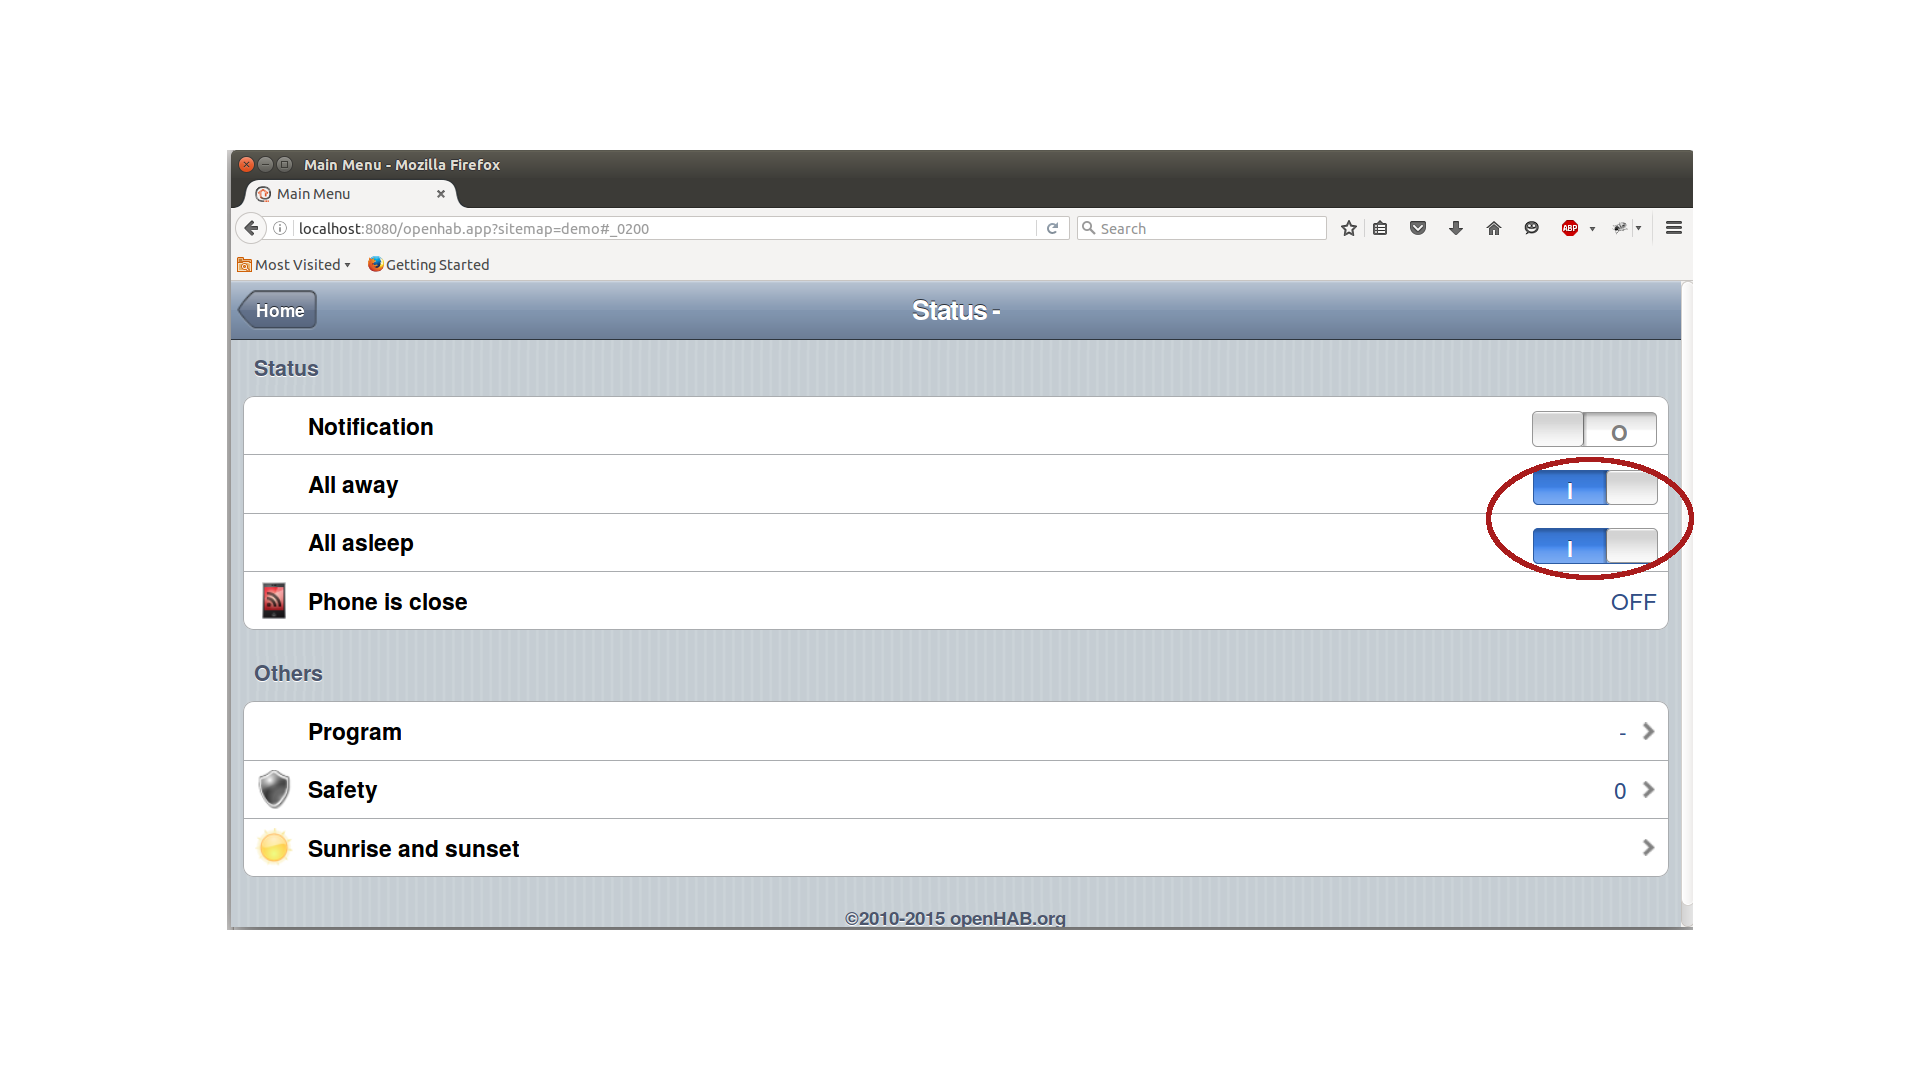
\includegraphics [trim=4cm 5cm 0 5cm, scale=0.14]{images/openhab-runtime.png}
\caption{Desktop UI showing that it is possible to set both \texttt{State\_Away} and \texttt{State\_Sleeping} to \texttt{ON} at the same time. Blue indicates that they are \texttt{ON}.}
\label{fig:awayrule}
\end{figure}
This example shows that even if the action block of a rule is implemented correctly, not having all the correct triggers can lead to too few firings of the rule and thus, unexpected behavior. To solve this problem, we propose a technique based on static analysis that can automatically generate event-based triggers and also detect missing ones by analysing code in the action block. 

\section{Threat model}
Since TrigGen can prevent incorrect behavior due to \textit{too few triggers}, it can also help eliminate security loopholes in the house that arise due to \textit{too few triggers}. Our approach can prevent any attack that relies on incorrect number of rule firings. One such example is described below with reference to the \texttt{Away rule} in section~\ref{sec:motivation}.

\textit{Example attack.} Smart homes often have a security notification system that sends a message to the owner's smart phone when there is someone at the door. There may be a rule (one possible rule is shown in listing~\ref{lst:security}) that activates the security notification system when everyone is away and deactivates it when everyone is sleeping at home. Since the "Away rule" in listing~\ref{lst:away} allows \texttt{STATE\_SLEEPING} to be set to \texttt{ON}  
when \texttt{STATE\_AWAY} is \texttt{ON}, firing it will wrongly deactivate the security notification system by triggering the rule in Listing~\ref{lst:security}. This will prevent the home inhabitants from knowing if there is an unwanted visitor in the house while they are away.
\begin{lstlisting}[caption={Rule for activating the security notification system in the house.},label={lst:security}]
rule "Security notification system rule"
when
  Item State_Away changed or
  Item State_Sleeping changed	
then
  if(State_Away.state == ON){
    postUpdate(Notification_System,ON)
  }
  if(State_Sleeping.state == ON){
    postUpdate(Notification_System,OFF)
  }
end
\end{lstlisting}

We assume that the action block of the rules is written correctly and rely on it for generating the trigger conditions.

We trust that the devices in the house are not compromised and once they receive a command, they execute it. We also trust the rule engine and the home automation OS for which the rules are written.

\section{\MakeLowercase{open}HAB background}
openHAB~\cite{openhab} is an open source software for integrating different types of smart devices in a home. openHAB has a runtime implemented in Java and a UI which can be used by end users for monitoring and controlling the devices. It supports 135 technologies, including more than 50 devices, cloud services like Twitter, DropBox, Google Calendar etc. and multiple communication protocols~\cite{openhabtech}. It has UI support for Android and iOS and an IFTTT integration~\cite{ifttt}. It is a java based solution which can be run on standard Linux, Windows and MacOS X machines as well as on embedded platforms such as Raspberry Pi and Cubietruck. It has about 50,000 downloads in the Google Play store with a rating of 4.4/5 and unlike most proprietary solutions, openHAB does not require any hardware installation and is completely technology and vendor agnostic, which makes it more accessible to home owners. 

The runtime provides a communication platform between the devices. 
%These are connected by means of an event bus. 
Figure~\ref{fig:framework} shows the main components of the openHAB framework. The item repository stores the states of the devices. It is connected to the UI and the rule base. Changes to the states can be made through the UI and by rule firings. The latest state is communicated to the actual device through the event bus. The bindings are libraries that connect the physical devices to the openHAB framework. As shown in the figure, there are two types of events that are communicated by the event bus---1) commands: causing an action or change of state in a device, such as \texttt{ON}, \texttt{OFF}, \texttt{UP}, \texttt{DOWN} and 2) updates: informing the UI component or the rule engine or other devices about a change in the state of a device.
\begin{figure}
\centering
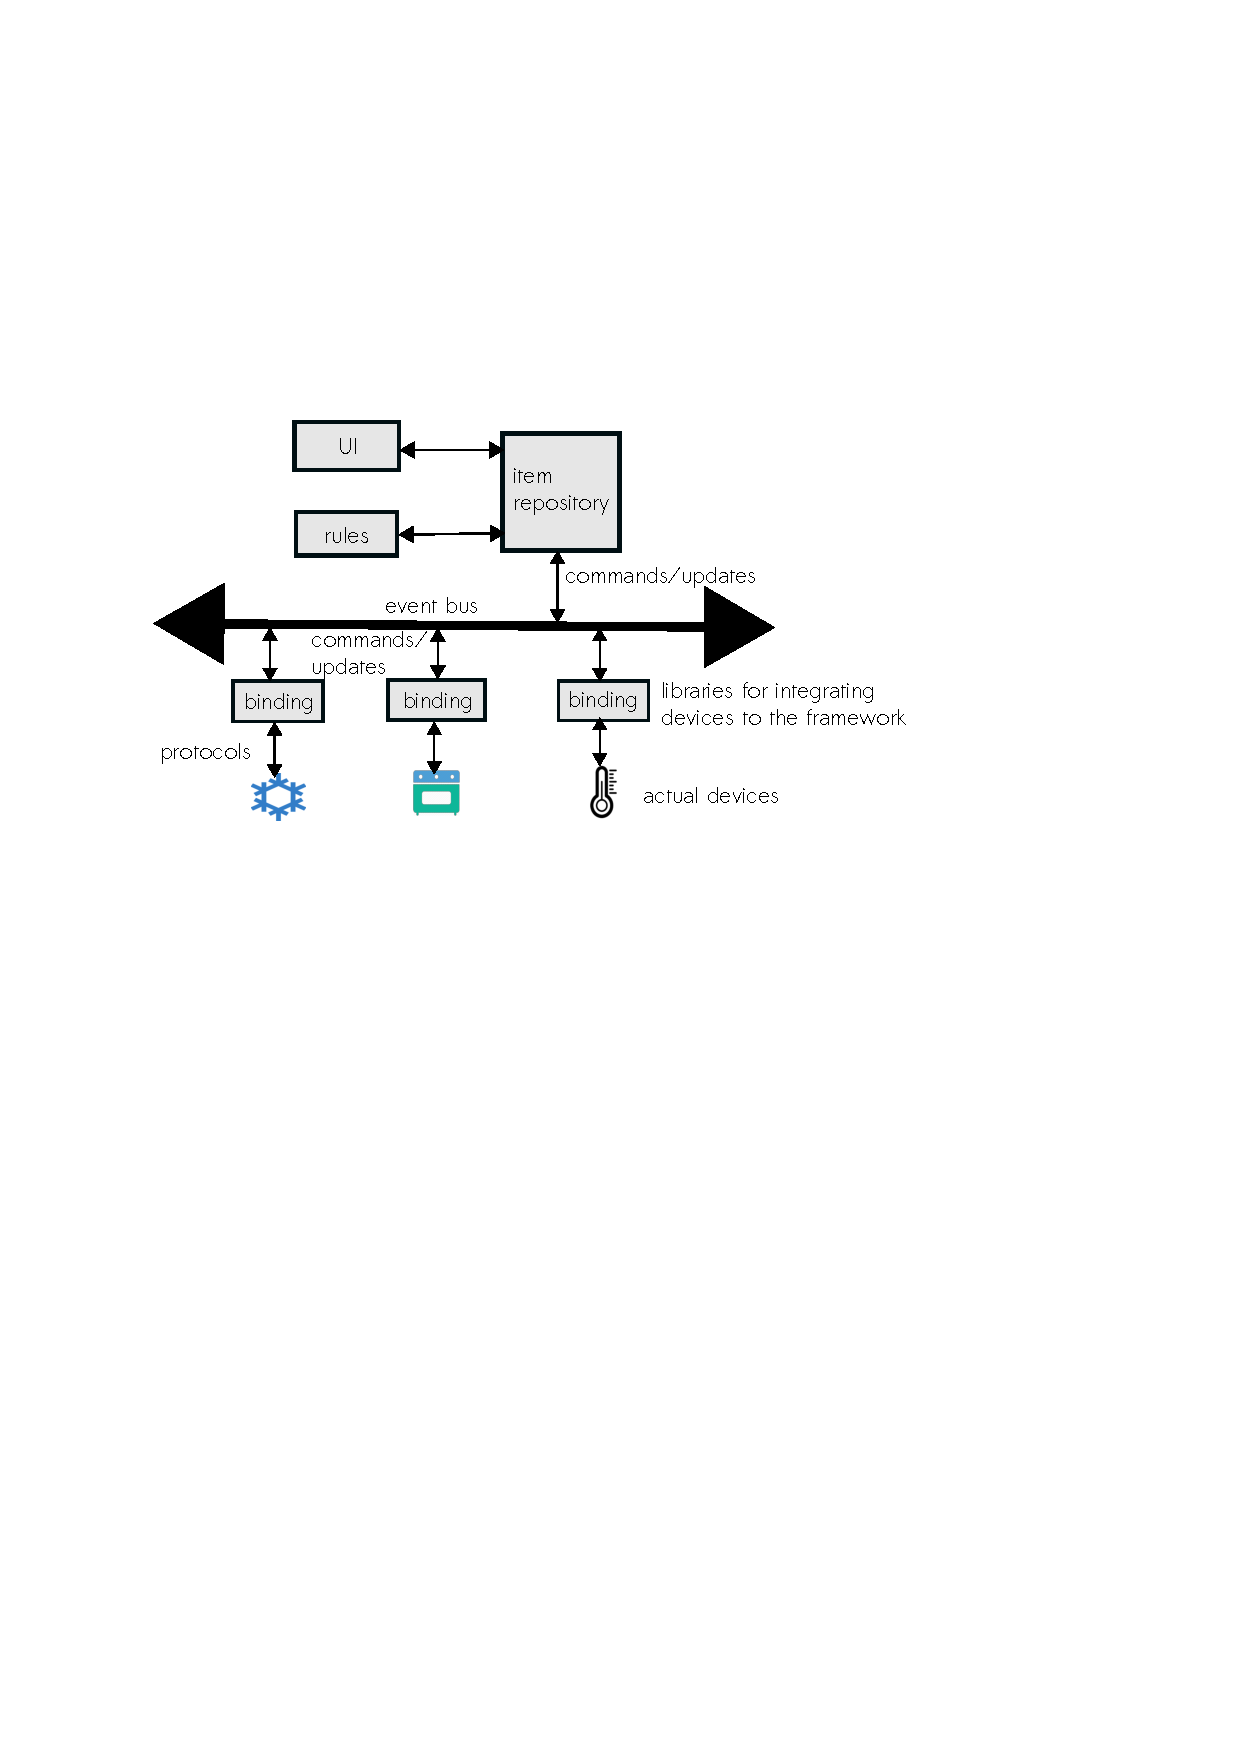
\includegraphics [trim=2cm 15cm 0 7.5cm, scale=0.6]{images/framework.pdf}
\caption{openHAB framework.}
\label{fig:framework}
\end{figure} 

End users can write the configuration files to customize the home. The main configuration files include a \textit{.rules} file containing the automation rules and an \textit{.items} file for storing the states of the devices installed. Each of these are written in small domain specific languages developed using the xtext framework~\cite{xtext}. The \textit{action block} in the rules, also called the \textit{script} is written in a Java like language called xbase, which is implemented using xtext. For our research, we required access to the item files and the rule files. 
\subsection{Items}
An item is any device installed in the house. There is an item file that contains a list of all items that are to be included in the automation. Every item has a type that indicates the values it can hold and the commands it can receive. Items can also be grouped together---all lights in the living room can be in one group so that they can be controlled together. An item may belong to multiple groups.
There are 11 types of items that are currently supported~\cite{openhabitem}. Listing~\ref{lst:items} shows the syntax of an item definition (contents in [~] are optional) and two entries in a sample item file. The binding part is responsible for connecting the item to an actual device ID.
\begin{lstlisting}[caption={Syntax and two examples of item definitions.},label={lst:items}]
<type> <name> ["label"] [<icon>] 
              [(group*)] [{binding}]
Switch DemoSwitch  "Switch"
Contact Window_Bedroom "Bedroom" 
        (Bedroom, Windows)
\end{lstlisting}
 
\subsection{Rules}
Listing~\ref{lst:rule} shows an example of a rule---it has two parts: a \emph{trigger block} and an \emph{action block}. The \emph{trigger block} can have one or more triggers. There are three types of triggers.
\begin{enumerate} [topsep=0pt,itemsep=-1ex]
\item event-based triggers: These triggers are related to changes in the state of a device. For examples---\\
\texttt{Item State\_Away changed}
\item temporal triggers: They cause rules to be fired at a certain time. 
\item system triggers: There are two system triggers---system start up and system shut down.
\end{enumerate}
The \emph{action block} of a rule in openHAB is also called the \emph{script}. It describes what the rule should do when the triggers occur.
\subsection{Actions}
\label{subsec:actions}
Actions are predefined methods that can be used in the \textit{action block} of a rule. The openHAB runtime provides a core set of actions but more can be implemented for specific devices by the respective manufacturers. The most important core actions for the purpose of our analysis are the event bus actions: \texttt{sendCommand(String itemName, String commandName)}, \texttt{postUpdate(String itemName, String stateValue)}. The entire list of actions can be found in the openHAB wiki~\cite{openhabwiki}. The \textit{action block} of a rule which is written in xbase, can invoke these actions. 

\section{Errors due to too few triggers}
\label{sec:theory}
\emph{Problem Definition}. Errors due to too few triggers is a condition where an insufficient number of triggers leads to fewer firing of a rule thereby leading to unexpected behavior or security vulnerabilities. \\

\emph{Goal}. Our goal is to prevent end users from making errors due to too few triggers---we want to ensure that all the correct triggers are included in the rules. \\

\emph{Approach}. Our approach is to automatically generate all the correct trigger conditions from the actions written by the end users. We developed a static technique to achieve this. Figure~\ref{fig:design} shows the design of our tool. It takes as input a \textit{rules} file and and \textit{items} file. The technique is explained below.
\begin{enumerate}
\item By statically analysing the AST of the script, $S$, we first identify all the items that appear in the action block of a rule, $R$. This is an exhaustive list of all potential event-based triggers. Let this list be $T$.
\item Naively adding all $t \in T$ as triggers of $R$ would either unnecessarily fire $R$ too many time or add redundant triggers which would make $R$ too complicated. Hence, we apply an elimination technique to get rid of triggers that are not required. The following definitions are used in the elimination algorithm. 

\emph{Definition 1}. An item is \emph{live} in $R$ if its value is read before it is written to in the rule script, $S$. 

\emph{Definition 2}. We define an item to be \emph{dependent} in $R$ if its value is computed based on other items or variables in the rule---this implies that the item is \emph{not live}. 
 
\emph{Definition 3}. We define an item to be \emph{independent} in $R$ if  its value is directly obtained from a sensor or a user's input and not computed based on any other item or variable---this implies that the item is \emph{live} in $R$. 

\emph{Definition 4}. We define an event-based trigger to be \emph{redundant} if inclusion of the trigger in a rule \emph{never} changes the state of any item or the value of any variable involved in $S$ when the rule is fired due to it.

\textbf{An item $d$ which is not \textit{live} in $R$ is not included in $T$ because it is redundant. As a corollary, if $d$ is dependent, it is also not included in $T$.}

\emph{Theorem}. If $d$ is not live in $R$, then it is a redundant trigger.\\
\emph{Proof}. Let us assume that $d$ is not redundant. That means it must change the value of some item or variable in $R$ in some firing. Let this item or variable be $a$. Since $d$ is not live, its value is never read before it is written to. The following cases are possible:
\begin{itemize} [topsep=-2pt, itemsep=-1pt]
\item $d$ is assigned a constant value. In this case, $d$ as a trigger does not change the value of $a$ because $d$'s value is always the same (as long as the script of R  itself is not changed).
\item $d$ is some function of other items, $i_1, i_2, ..., i_n$ and variables $v_1, v_2, ..., v_m$ in $R$. In this case, $d$ as a trigger will still not affect the value of $a$ because $d$'s own value depends on the values of items $i_1, i_2, ..., i_n$---a will change only if the values of the live items from $i_1, i_2, ..., i_n$ change. Hence, adding them as triggers would be sufficient.
\end{itemize}
This shows that $d$ never causes the value of $a$ to change. Therefore, our assumption that $d$ is not redundant is wrong. Hence, $d$ must be redundant. $\blacksquare$
\end{enumerate}

\noindent \emph{Enumerating groups}. Items can be grouped so that they can be controlled together if needed---the rule scripts can perform operations on all the member items of a group. Listing~\ref{lst:group} shows examples of groups in an \textit{items} file.
A group can have multiple items and one item can belong to one or more groups. Groups can also be contained in other groups. For such rules, TrigGen generates triggers by enumerating all members of a group. It performs a depth first search to determine all the groups to which an item belongs. Figure~\ref{fig:graphstructure} shows the graph representing the items in listing~\ref{lst:group}. 
\begin{lstlisting}[caption={Grouping of items (GF stands for Ground Floor).},label={lst:group}]
Group All
Group GF(All)
Group GF_Living(GF) 										
Group Lights(All)
Dimmer Light_GF_Living(GF_Living,
                       Lights)
\end{lstlisting}
\begin{figure}
\centering
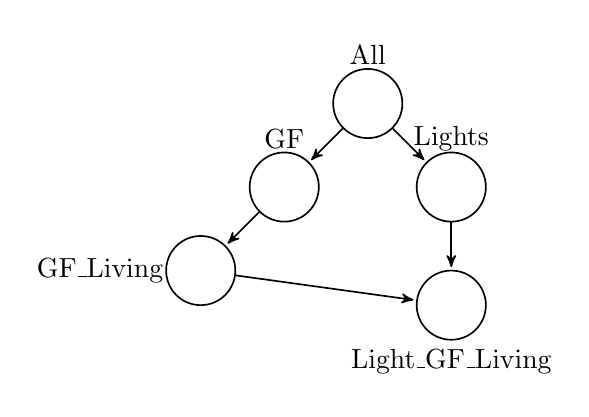
\begin{tikzpicture}[->,>=stealth',shorten >=1pt,auto,node distance=1.5cm,
                    semithick,minimum size=2em]
  \tikzstyle{every state}=[fill=white,draw=black,text=black]

  \node[state, label={[label distance=-0.2cm]90:All}]         (A)  {};  
  \node[state, label={[label distance=-0.2cm]90:GF}] 		(B) [below left of=A] {};  
  \node[state, label={[label distance=-0.2cm]90:Lights}]         (C) [below right of=A] {};
  \node[state, label={[label distance=-0.1cm]180:GF\_Living}]         (D) [below left of=B] {};
  \node[state, label ={[label distance=-0.1cm]270:Light\_GF\_Living}]         (E) [below of =C] {};

  \path (A) edge              node {} (B)
            edge              node {} (C)            
        (B) edge              node {} (D) 
        (D) edge				 node {} (E)          
        (C) edge 			 node {} (E);             
\end{tikzpicture}
\caption{Graph representing the item grouping shown in listing~\ref{lst:group}}
\label{fig:graphstructure} 
\end{figure}
\noindent \emph{Conflict resolution}. If there are multiple rules that modify the state of the same item, then TrigGen warns the users about a potential conflict. Consider the rule written by an end user in listing~\ref{lst:conflict} as an example. Before \texttt{Air\_G\_Message} is updated, its current value is checked against \texttt{msg}. If there is another rule, say $R'$ that writes to \texttt{Air\_G\_Message}, then there could be a conflict between this rule and $R'$. TrigGen detects such conflicts and warn the end user about the possibility of a conflict. It is then upto the user to determine the severity of the warning and whether the rules need to be corrected.
\begin{lstlisting}[caption={Rule for updating the status message for the air quality in the garage.},label={lst:conflict}]
rule "Air garage"
when
 Item Temp_G changed
 or
 Item Humidity_G changed
then
 if(Temp_G.state != null && 
    Humidity_G.state != null){
     var String msg = Temp_G.state.toString()
                + Humidity_G.state.toString()
     if(Air_G_Message.state != msg){
      postUpdate(Air_G_Message,msg)
     }
 }
end
\end{lstlisting}

\begin{figure*}
\centering
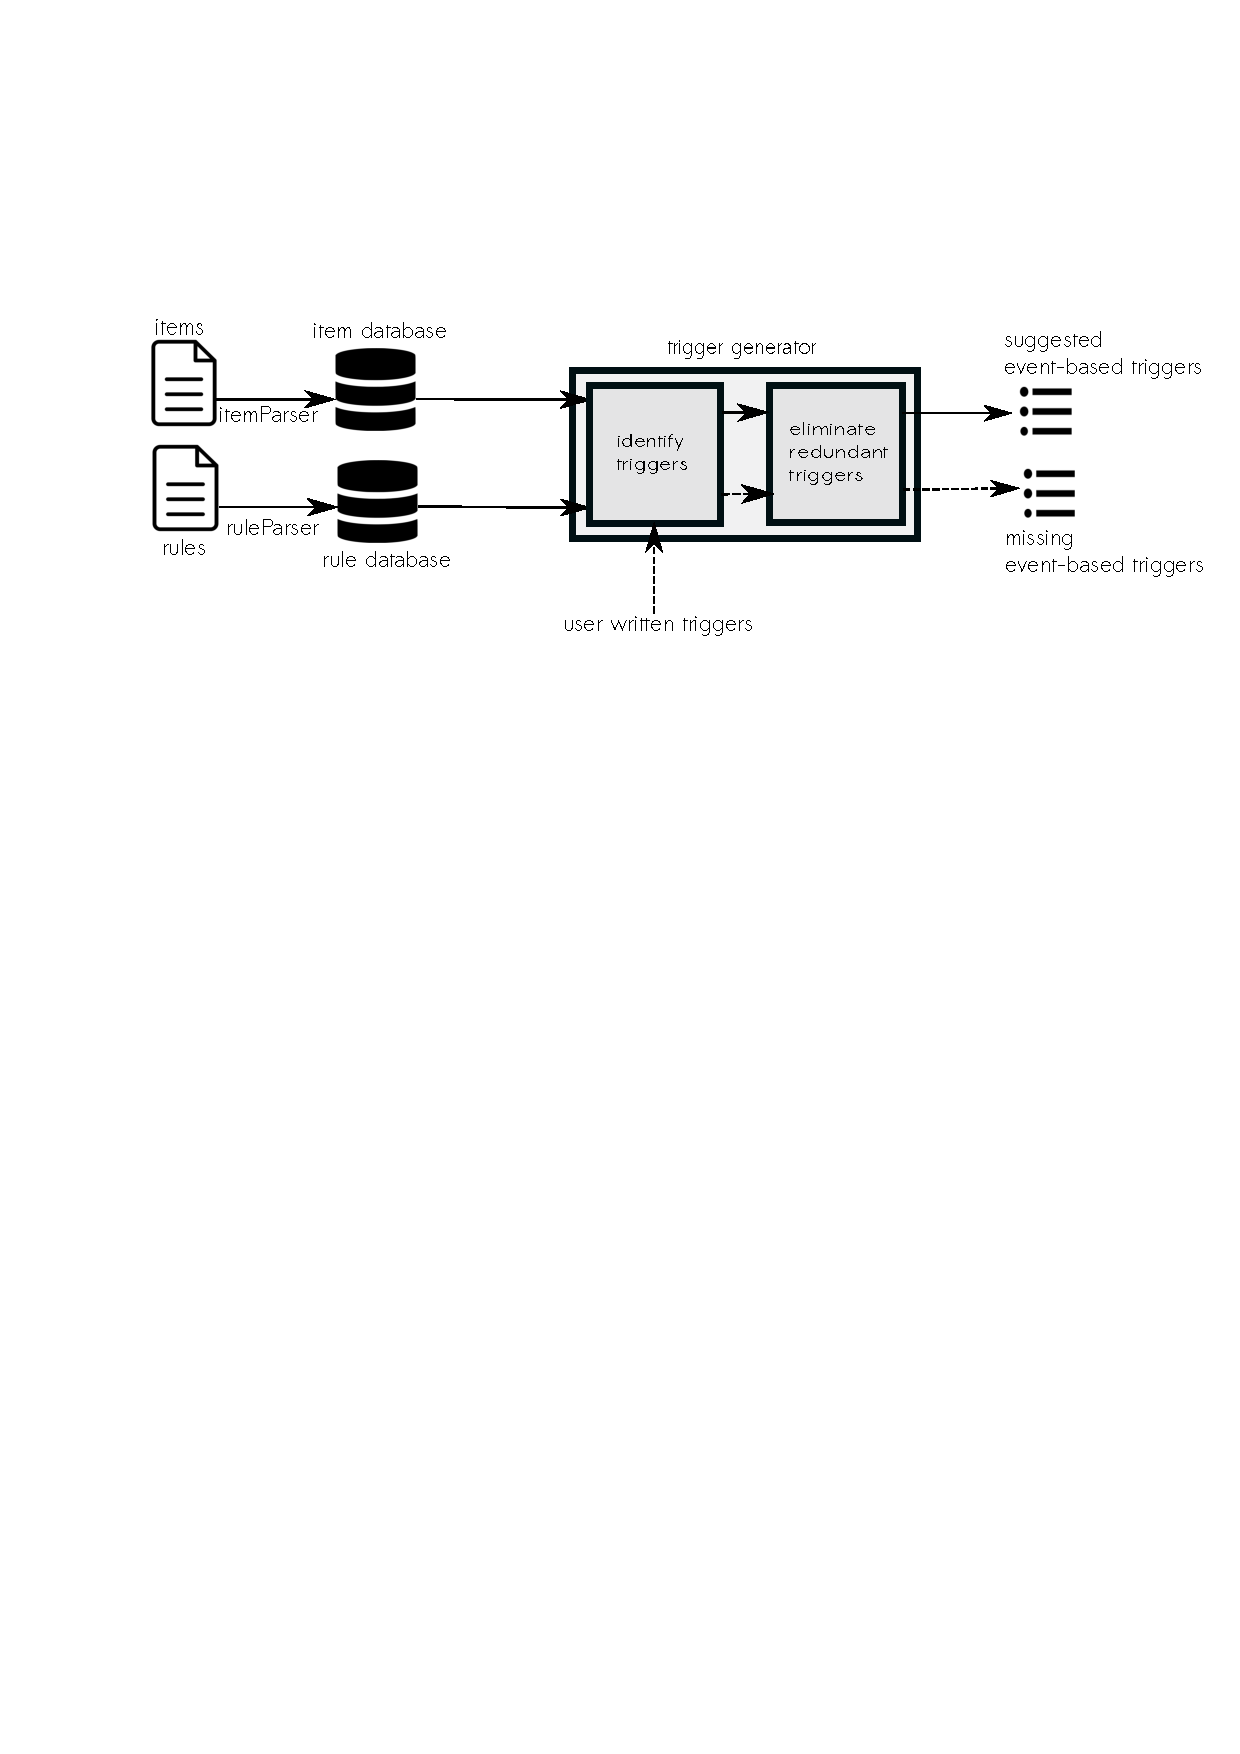
\includegraphics [trim=0cm 18cm 0 5cm, scale=0.8]{images/design.pdf}
\caption{Design of the TrigGen tool.}
\label{fig:design}
\end{figure*} 

\section{Implementation}
We implemented TrigGen in Java. It involved $\sim$ 3500 LOC. Our tool can be used directly on a rule file without any pre-processing or annotations from the end users. 

Figure~\ref{fig:design} shows the design of TriGen. We generated parsers for the rules and items using the respective grammars provided by openHAB. For this, we used the xtext language tools~\cite{xtext}. We stored the item information such as item names, types, and groups they belong to, in an item database. For the rules, we used the AST generated by xtext and visited the nodes in it to extract the names of the device states appearing in assignments, as actual method arguments, conditions in if-statements, closures and all other language constructs supported by the rule DSL. We stored this information in a rule database. 

The next step is the trigger generation in which all device states are first naively added to the list of potential triggers. This list is then analysed to eliminate the redundant triggers as explained in section~\ref{sec:theory} to generate a list of necessary and sufficient triggers. 

The list of generated triggers is compared with the triggers written by the end users if any, to detect the missing/extraneous ones.

TrigGen also identifies rules which might conflict with each other due to modifying the state of the same device. 

 
\section{Experimental Evaluation}
We evaluated TrigGen on 116 end user written rules. We obtained the rules from links provided on the openHAB wiki~\cite{data1},\cite{data2}. We ran TrigGen on a machine running 64 bit Ubuntu 14.04 LTS with 2.6 GHz quad core processor. Table~\ref{tab:time} shows the time taken for TrigGen to complete executing.
For 109 out of the 116 rules (94\%), TrigGen suggested a list of all required event-based triggers and for 77 out the 116 rules (66\%), it found missing triggers when some triggers were already provided by the users. For 19 rules (16\%), TrigGen generated warnings about potential conflicts. 

\begin{table}[ht]
\centering
\begin{tabular}{|l|c|}
\hline
Action & Execution time\\ \hline
generate all triggers & 6.88 s \\ \hline
detect missing triggers & 7.31 s \\\hline
\end{tabular}
\caption{Execution time  (in seconds) summary of TrigGen for 116 rules for 1) generating all event-based triggers, and 2) detecting missing triggers. }
\label{tab:time}
\end{table}

Figure~\ref{fig:resultgraph} shows the output of TrigGen for generating the necessary and sufficient set of triggers. As is evident from the figure, for majority of the rules, TrigGen suggested 2 event-based triggers and detected 1 missing trigger. The large number of triggers which were determined for some rules (as shown in figure~\ref{fig:resultgraph}) was due to the grouping of items. TrigGen expanded the groups as explained in section~\ref{sec:theory} to enumerate all the contents of the groups. 

All the triggers that TrigGen detected as \textit{missing} were true positives. If the triggers written by the end users only include system and temporal triggers, then TrigGen does not suggest any other event-based trigger because that would modify the behavior of the rule. If however, at least one event-based trigger is included, then it detects those event-based triggers that are missing. 
Table~\ref{tab:scope2} summarizes the output of TrigGen for identifying missing triggers. 
\begin{table}[ht]
\centering
\begin{tabular}{|l|p{4cm}|}
\hline
user written triggers & tool's output \\ \hline
at least one event-based & \parbox[t]{5cm}{missing event-based triggers, \\extraneous triggers}  \\ \hline
only temporal and/or system & none \\\hline
\end{tabular}
\caption{Output of TrigGen for detecting missing triggers when some triggers are already written by the user.}
\label{tab:scope2}
\end{table}

For 2 out of the 7 rules for which TrigGen did not \textit{suggest} any event-based triggers, we compared the report with the triggers written by the end user. We found that the triggers were System triggers---the rules were supposed to be fired only once at system start-up. Hence TrigGen's output was correct because it did not suggest any event-based triggers. 

\textbf{Limitations.}
By comparing the suggested trigger for the 109 rules with the triggers written by the end user, we found that for 20 of them the  event-based triggers suggestions from TrigGen were incorrect. This was because for these 20 rules, the end user only expected temporal or system triggers while TrigGen is a tool for generating event-based triggers only.

For 5 rules TrigGen failed to suggest triggers due to two reasons---1) since TrigGen uses the AST of the rule script to extract items that can be potential triggers, if there is no reference to an item in the script, TrigGen cannot detect the trigger. This happened in 4 out of the 5 cases. 2) For the remaining one case, the item suggested by the end user as a trigger is read from using a \todo{need to consider this one case where the tool fails} . According to our technique, such items are considered non-live and not included in the list of triggers. As a result, TrigGen failed to identify it.

\begin{figure*}[t]
\centering
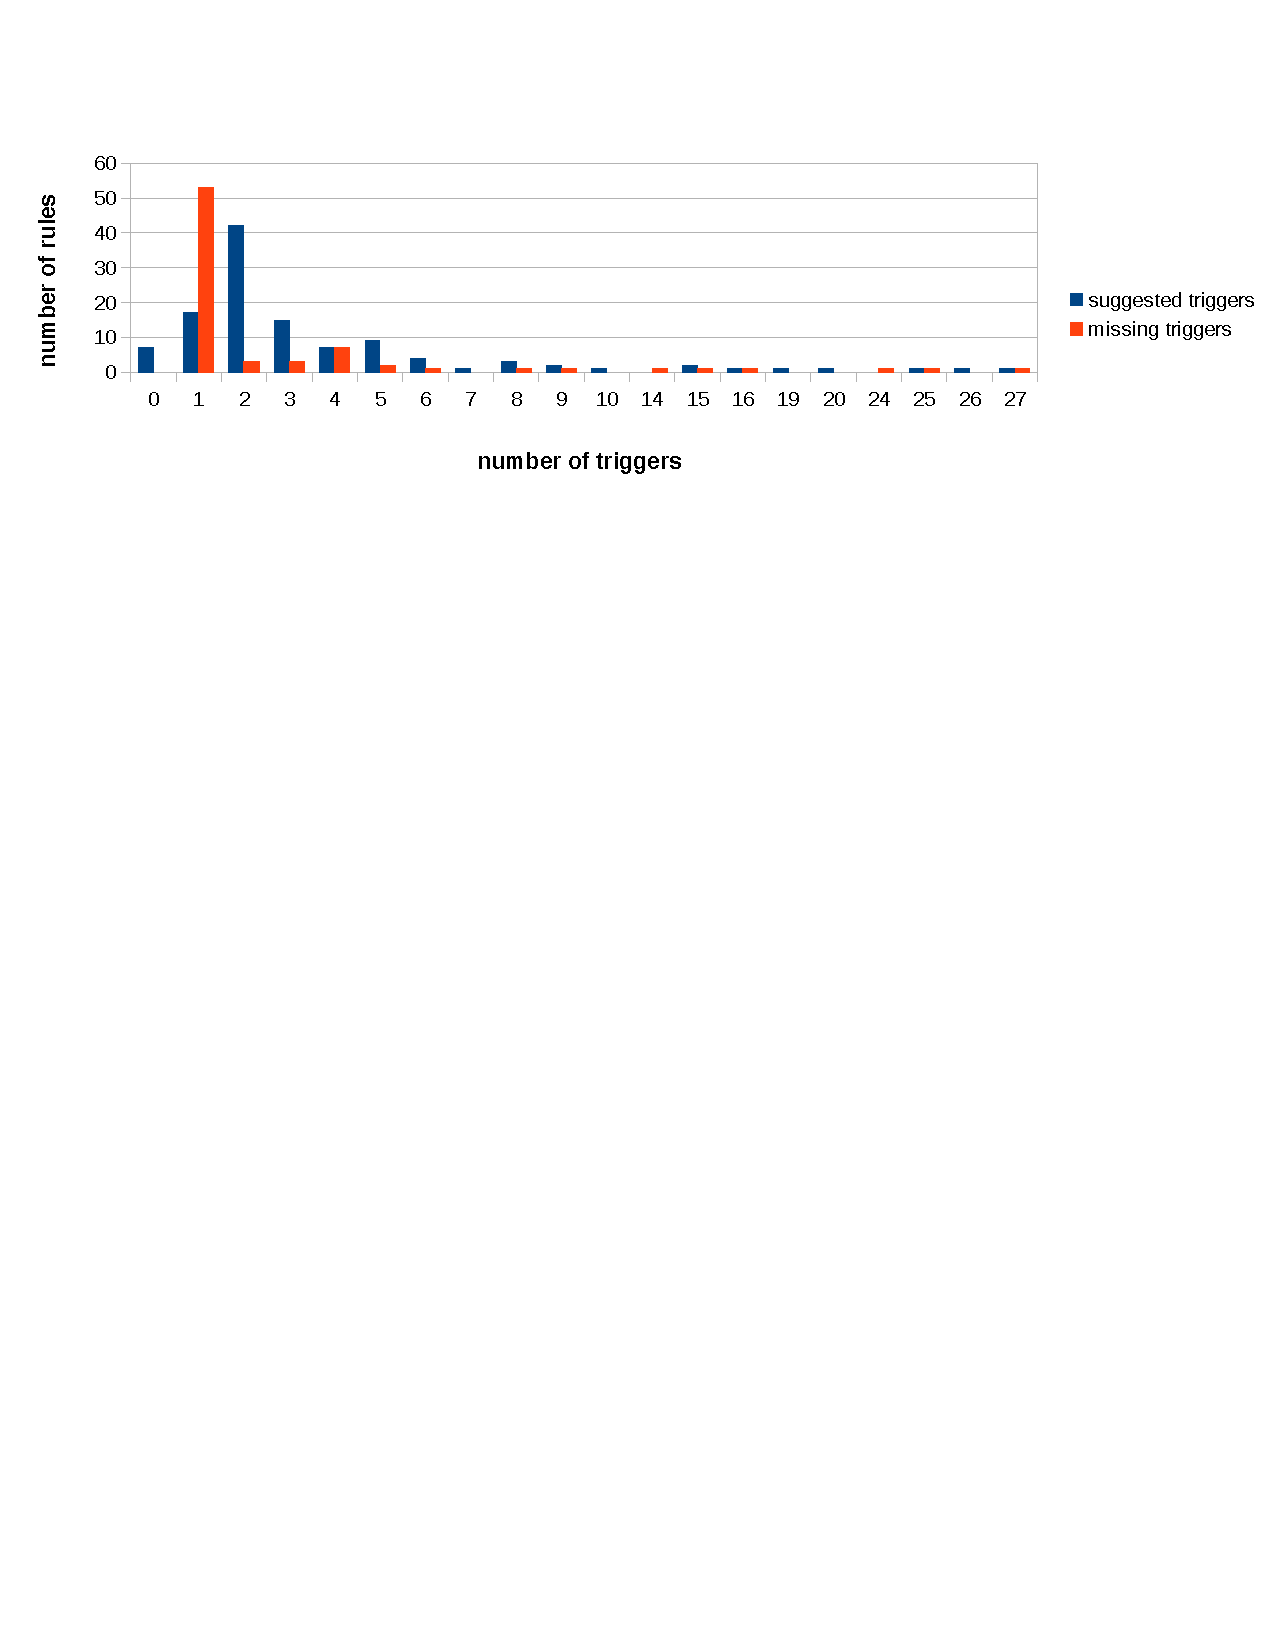
\includegraphics [trim=10 500 50 90, scale=0.7]{images/plot.pdf}
\caption{Summary of the output of TrigGen for suggesting a set of necessary and sufficient triggers (in black) and detecting missing triggers (in red). The x-axis shows the number of suggested triggers and the y-axis shows the number of rules.}
\label{fig:resultgraph}
\end{figure*} 

Table~\ref{tab:scope1} summarizes the usefulness of our tool for suggesting triggers with respect to the conditions under which the user actually expects the rule to be fired.
\begin{table}[ht]
\centering
\begin{tabular}{|l|l|}
\hline
user's expectation & usefulness \\ \hline
event-based & high \\ \hline
temporal & low \\\hline
system & low \\ \hline
\end{tabular}
\caption{Usefulness of TrigGen for suggesting triggers only based on the rule script (no triggers written by the user)---\textit{high} indicates that all the suggestions are useful and \textit{low} indicates that none of the suggestions are useful. }
\label{tab:scope1}
\end{table}

\section{Related work}
Security goals and potential vulnerabilities in smart homes have been investigated in several papers~\cite{yoshi, dhanjani, jung, todayToTomorrow}. Denning et al.~\cite{yoshi} identified assets within a home that are susceptible to security attacks and suggested security goals for smart homes. Ur et al.~\cite{jung} conducted a case study of three specific smart devices to analyse the state of access control for home automation. Mennicken et al.~\cite{todayToTomorrow} studied the importance of human-home-collaboration in making smart homes more accessible.

Recently, Fernandes et al.\cite{smartthings16} did a security analysis of several apps based on Samsung SmartThings and discovered that many of them unnecessarily granted full access to the devices in the house. While they aimed at identifying security flaws in the SmartThings framework itself, our aim is to assist end users in writing correct automation rules and we do so by automatically generating the trigger conditions.  Further, instead of analysing apps for home automation, we analysed end user written automation rules.

Some work has been done on detecting conflicts in trigger-action programs~\cite{rvs, homer, utea, Nakamura05featureinteractions}. TrigGen's main capability is to automatically generating the correct triggers for a rule although it can also identify rules which can potentially have conflicts. None of the previous tools can automatically determine trigger conditions.

The usefulness of TAP for customizing smart homes has been studied by Ur et al.~\cite{practical-tap} and Dey et al.~\cite{dey}. Their findings motivated us to focus on end user written rules for home automation---they showed by conducting user studies that about 80\% of the automation requirements of the users could be represented by trigger action programs~\cite{dey} and even non-programmers could easily learn TAP~\cite{practical-tap}.

Huang et al.~\cite{Huang} conducted user studies on TAP to identify inconsistencies in interpreting the behavior of a trigger action programs and errors in writing them and found that often the interpretation of a rule by a user is different from the semantics of the rule. 

One of the observations in some recent work is that the IFTTT framework~\cite{iftttframework} which only allows single trigger is not sufficient for expression complex automation rules for smart homes~\cite{Huang, practical-tap}. This motivated us to evaluate our tool on the openHAB framework which has a more expressive rule language allowing multiple triggers. 


\section{Conclusions}
End users have a major role in home automation---they decide the automation rules for the devices. Not surprisingly, our research shows that these end user written rules are often error-prone.
We observed that a common error made by end users while writing the rules is having insufficient number of triggers, leading to fewer firings of the rules than necessary. To prevent this problem, we developed TrigGen that can automatically generate a set of necessary and sufficient triggers based on the actions in a rule. This also reduces the burden of end user by assisting them in writing the necessary and sufficient triggers. 

We evaluated TrigGen on real home automation rules written by end users and found that out of 116 rules, 77 had insufficient number of triggers. By manual inspecting the suggestions provided by the tool, we found that each one of them were relevant and including them in the rules prevented the unexpected behaviors observed previously. 


\section{Acknowledgements}
We thank Franziska Roesner for her valuable feedback and Jeanette Daum for contributing to an earlier version of this project.
\bibliographystyle{abbrv}
\bibliography{sigproc}  

\end{document}
